\documentclass{beamer}
\usepackage{amsfonts}
\usepackage{amsmath}
\usepackage{times}
\usepackage{mathrsfs}
\usepackage{extarrows}
\usepackage{bbm} 
\setbeamercolor{footcolor}{fg=blue!100} % 设置字体和背景颜色
\setbeamertemplate{headline}{%
  \leavevmode%
  \hbox{%
    \hskip228pt
    \begin{beamercolorbox}[wd=.126\paperwidth,ht=2.25ex,dp=1ex,right]{footcolor}%      
       \textcolor[rgb]{0,0.168,0.376}{Slide \insertframenumber{} }
    \end{beamercolorbox}}%
  \vskip-19pt%
}

\setbeamertemplate{frametitle}
{
\vspace{30pt}\textcolor[rgb]{0,0.168,0.376}{\insertframetitle}
}

 
\pgfdeclareimage[height=0.61cm]{university-logo}{logo.png}  
\logo{\pgfuseimage{university-logo}{\vspace{244pt}}} 
\title{\textcolor[rgb]{0,0.168,0.376}{VV286 Review 2}}
\author{JIANG Yicheng}
\begin{document}

\begin{frame}
\titlepage
\end{frame}

\begin{frame}
\begin{block}{Evaluation of Real Integrals}
$$\int_{\mathbb{R}/\mathbb{R}^+}f(x)dx=A$$
\begin{enumerate}
\item Extend the real domain to complex domain.
\begin{enumerate}
\item Usually you only need to change $x\in \mathbb{R}$ to $z\in\mathbb{C}$
\item For $\sin x, \cos x$, do integral for $e^{iz}$
\end{enumerate} 
\item Find poles for the function $f(z)$


\item Decide the contour and the branch (for $x^{\alpha},\ln x$) if needed.
\item Calculate the residue for poles in the contour.
\begin{enumerate}
\item During an exam, you may calculate residue for all poles if you cannot decide the contour at first.
\end{enumerate}
\item Apply residue theorem or Cauchy's theorem.
\end{enumerate}
\end{block}
\end{frame}

\begin{frame}
$$\int_{\mathcal{C}}f(z)dz=2\pi i\sum\limits_{k=1}^N\text{res}_{z_k}f$$
\begin{block}{For right hand side}
$$\text{res}_{z_0}f=\dfrac{1}{(n-1)!}\lim_{z\rightarrow z_0}\dfrac{d^{n-1}}{dz^{n-1}}\big((z-z_0)^nf(z)\big)$$
$$\text{RHS}=a_1+b_1i$$
\end{block}
\begin{block}{For left hand side}
$$\text{LHS}=A+0+a_2+b_2i+(a_3+b_3i)A$$
$$\text{LHS}=\text{RHS}\Rightarrow A=\dfrac{a_1-a_2}{1+a_3}$$
\end{block}
\end{frame}

\begin{frame}
\begin{block}{Singularities}
Let $\Omega\subset\mathbb{C}$ be \textcolor[rgb]{0,0.6,0.3}{\textbf{\textit{open}}}, $z_0\in\Omega$ and $f:\Omega\setminus\lbrace z_0\rbrace\rightarrow\mathbb{C}$ holomorphic. Then $f$ is said to have a point singularity or isolated singularity at $z_0$.
\begin{enumerate}
\item The singularity is said to be removable if there exists an analytic continuation $\tilde{f}:\Omega\rightarrow\mathbb{C}$. (such $\tilde{f} $ is unique)
\item The singularity is said to be a \textcolor[rgb]{0,0.6,0.3}{\textit{\textbf{pole}}} if $g=1/f$ is holomorphic on $\Omega\setminus\lbrace z_0\rbrace$ and has a removable singularity at $z_0$ such that the analytic continuation $\tilde{g}$ of $g$ satisfies $\tilde{g}(z_0)=0$.
\item The singularity is said to be essential if it is neither removable nor a pole.
\end{enumerate}
\end{block}
\end{frame}


\begin{frame}
\begin{block}{How to judge? }

\end{block}
\begin{block}{Removable Singularity}
Whether $\lim\limits_{z\rightarrow z_0}f$  exists.

e.g. 
$$\lim\limits_{z\rightarrow0}\dfrac{\sin z}{z}=1$$
So $f(z)=\dfrac{\sin z}{z}$ has removable singularity at $z=0$.
\end{block}
\begin{block}{Pole (Informal way)}
$f(z)=\dfrac{g(z)}{h(z)}$, then all $z_0$ such that $h(z_0)=0$ may be a pole.

 (All $z_0$ such that $g(z_0)=0$ may be a zero.)
\end{block}
\end{frame}

\begin{frame}
\begin{block}{Multiplicity of Poles}
If $f : \Omega\mapsto\mathbb{C}$ has a pole at $z_0\in\Omega$, then in a neighborhood $U$ of that point there exist a non-vanishing holomorphic function $h$ and a unique positive integer $n$ such that
$$f(z)=(z-z_0)^{-n}h(z)\hspace{5mm}\text{for all}\,\, z\in U$$
The integer $n$ is called the multiplicity
or order of the pole of $f$ . If $n = 1$, we say that the pole is \textcolor[rgb]{0,0.6,0.3}{\textbf{\textit{simple}}}.
\end{block}
\begin{block}{}
$$f(p)=\dfrac{p+e^{-\frac{\pi}{2}p}}{(1+p^2)^2}$$

\end{block}

\end{frame}
\begin{frame}
\begin{block}{Principle Part}
\begin{align*}
f(z)&=(z-z_0)^{-n}\sum\limits_{m=0}^{\infty}b_m(z-z_0)^m\\
&=\dfrac{b_0}{(z-z_0)^n}+\dfrac{b_1}{(z-z_0)^{n-1}}+\cdots+\dfrac{b_{n-1}}{z-z_0}+\sum\limits_{m=n}^{\infty}b_m(z-z_0)^{m-n}\\
&=\underbrace{\dfrac{a_{-n}}{(z-z_0)^n}+\dfrac{a_{-(n-1)}}{(z-z_0)^{n-1}}+\cdots+\dfrac{a_{-1}}{z-z_0}}_{\text{Principle part}}+\sum\limits_{m=0}^{\infty}a_0(z-z_0)^m
\end{align*}
$a_{-1} $ is the residue of $f$ at $z_0$
\end{block}
\end{frame}

\begin{frame}
\begin{block}{Contour 1----Semi-circle}
\begin{figure}[h]
    \centering
    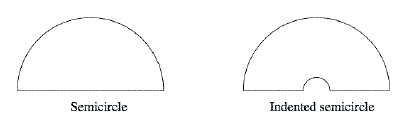
\includegraphics[width=10cm]{semicircle.png}
\end{figure}
Most common ones.

You have used them to solve 
$$\int_0^{\infty}\dfrac{\sin x}{x}dx,\,\,\,\,\int_{-\infty}^{\infty}\dfrac{\cos x}{x^2+a^2}dx,\,\,\,\,\int_{-\infty}^{\infty}\dfrac{x\sin x}{x^2+a^2}dx,\,\,\,\,\int_{-\infty}^{\infty}\dfrac{dx}{1+x^4}$$
$$\int_0^{\infty}\dfrac{x\sin x}{(x^2+4)^2}dx,\,\,\,\,\int_{-\infty}^{\infty}\dfrac{dx}{(1+x^2)^{n+1}}dx,\,\,\,\,\int_{0}^{\infty}\dfrac{1-\cos x}{x^2}dx$$
\end{block}
\end{frame}

\begin{frame}
\begin{block}{Contour 2----Sector}
\begin{figure}[h]
    \centering
    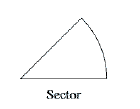
\includegraphics[width=4cm]{sector.png}
\end{figure}
Similar to Semi-circle.

May be useful for integral containing $\sin(x^n)$, $\cos(x^n)$ 

(choose central angle=$\dfrac{\pi}{2n}$) 

You have used it to solve 
$$\int_0^{\infty}\sin x^2dx,\,\,\,\,\int_{0}^{\infty}\cos x^2dx$$
\end{block}
\end{frame}

\begin{frame}
\begin{block}{Contour 3}
\begin{figure}[h]
    \centering
    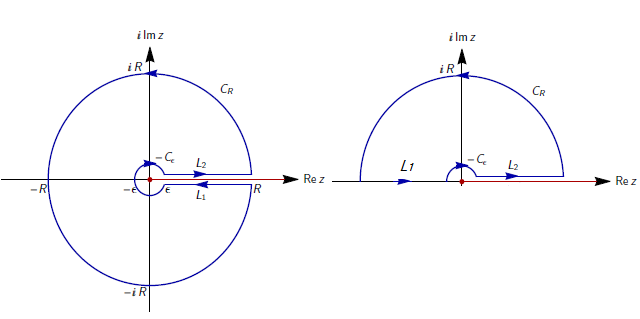
\includegraphics[width=10cm]{branch.png}
\end{figure}

Used for integral containing $\sqrt{x}$, $\ln x$ (For these two contours, the branch we choose is $\mathbb{C}\setminus\mathbb{R}^0_-$, so $\phi\in(0,2\pi)$)

$$\int_0^{\infty}\dfrac{\sqrt{x}}{x^2+a^2}dx,\,\,\,\,\int_{0}^{\infty}\dfrac{\ln x}{x^2+a^2}dx$$
\end{block}
\end{frame}


\begin{frame}
\begin{block}{Residue Calculus for Functions with Branch Points}
Let $P$ and $Q$ be polynomials of degree $m$ and $n$, respectively, where $n\geqslant m+2$. If $Q(x)\neq0$ for $x>0$, if $Q$ has a zero of order at most 1 at the origin and if
$$f(z)=\dfrac{z^{\alpha}P(z)}{Q(z)},\hspace{3mm}0<\alpha<1$$
then
$$\text{p.v.}\int_0^{\infty}\dfrac{x^{\alpha}P(x)}{Q(x)}dx=\dfrac{2\pi i}{1-e^{2\pi \alpha i}}\sum\limits_{j=1}^k\text{res}_{z_j}f$$
\end{block}
This theorem is obtained by using the contour in the left on last slide. Pay attention to the branch. Also pay attention to its requirement. 
\end{frame}

\begin{frame}
\begin{block}{Contour 4}
\begin{figure}[h]
    \centering
    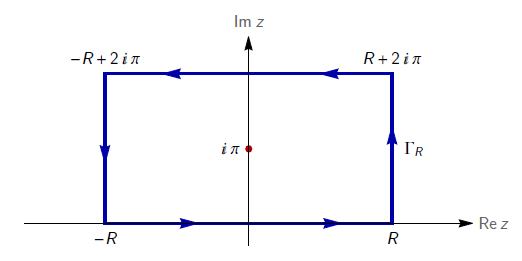
\includegraphics[width=8cm]{rectangle.png}
\end{figure}

$$\int_0^{\infty}\dfrac{e^{ax}}{1+e^x}dx$$
\end{block}
\end{frame}


\begin{frame}
\begin{block}{Lapalace Transform}
$$(\mathscr{L} f)(p)=\int_0^{\infty}e^{-pt}f(t)dt$$
$$\text{Convolution}: (\mathscr{L})^{-1}\Big((\mathscr{L}f)\cdot(\mathscr{L} g)\Big)=f*g=\int^t_0f (t-s)g(s) ds$$
$$\text{Bromwich Integral: }(\mathscr{M}F)(t) =\dfrac{1}{2\pi i}\int_{\beta-i\infty}^{\beta+i\infty}e^{pt}(\mathscr{L} f)(p) dp$$

\end{block}
\begin{block}{Fourier Transform}
$$\widehat{f}(\xi)=\dfrac{1}{\sqrt{2\pi}}\int_{-\infty}^{\infty}f(x)e^{-i\xi x}dx$$
$$f(x)=\dfrac{1}{\sqrt{2\pi}}\int_{-\infty}^{\infty}\widehat{f}(\xi)e^{i\xi x}d\xi$$
\end{block}
\end{frame}


\begin{frame}
\begin{block}{Solving an ODE with the Laplace Transform}
To deal with discontinuous inhomogeneities and even inhomogeneities that are not functions at all.
$$ay''+by'+cy=f(x),\,\,\,y(0)=y_0,\,\,\,y'(0)=y_1$$
\end{block}
\begin{block}{1.}
Apply the Laplace transform to both sides of the ODE/IVP;
\begin{align*}
(\mathscr{L}f')(p)&=p\cdot(\mathscr{L}f)(p)-f(0)\\
(\mathscr{L}f'')(p)&=p^2(\mathscr{L}f)(p)-p\cdot f(0)-f'(0)
\end{align*}
$$(ap^2+bp+c)Y-(ap+b)y_0-ay_1=(\mathscr{L}f)(p)$$
\end{block}
\end{frame}

\begin{frame}
\begin{block}{2.}
$$Y=(\mathscr{L}f)(p)\cdot\dfrac{1}{ap^2+bp+c}+\dfrac{ay_0p+by_0+ay_1}{ap^2+bp+c}$$
Find $g(x)$ such that $(\mathscr{L}g)(p)=\dfrac{1}{ap^2+bp+c}$

The function $g$ is called a Green's function for the differential
equation.
\end{block}
\begin{block}{3. }
Use transform table and apply convolution to find inverse Laplace transform.
\end{block}
\end{frame}

\begin{frame}
\begin{block}{Note}
\begin{enumerate}
\item Since we usually need to use convolution to find inverse Lapalace transform, we don't need to take Lapalace transform for those on the right hand side of the equation.
\item If $f$ or $g$ contains $H(x)$, don't insert $x-s$ into $H(x)$
\end{enumerate}
\end{block}
\end{frame}
\begin{frame}
\begin{block}{Calculate the Fourier transform}
\begin{enumerate}
\item Do direct integral
\item Do direct integral through contour integration in
the complex plane
\item Construct ODE 

\end{enumerate}

\end{block}
\end{frame}

\begin{frame}
\begin{block}{Solving an ODE with the Fourier Transform}
$$ay''+by'+cy=f(x) $$
We do not impose any initial conditions but instead require that
$$\lim\limits_{x\rightarrow\pm\infty}y(x) = 0$$
and assume that $y$ is absolutely integrable.

\end{block}

\end{frame}





\begin{frame}
\begin{block}{Decay}
Let $\Omega \subset \mathbb{R}$ be bounded and $f : \mathbb{R}\setminus \Omega
\rightarrow \mathbb{C}$.
\begin{enumerate}

\item  If $ f (x) = O(x^{-n})$ as $|x|\rightarrow\infty$  for some $n > 0$, then $f$ is said to have polynomial decay at infinity.
\item  If $ f (x) = O(x^{-n})$ as $|x|\rightarrow\infty$ for all $n > 0$, then $f$ is said to have faster-than-polynomial decay at infinity.
\item  If $ f (x) = O(e^{-b|x|})$ as $|x|\rightarrow\infty$ for some $b > 0$, then $f$ is said to have exponential decay at infinity.
\end{enumerate}
\end{block}
\end{frame}




\end{document}
